\chapter{BERT}

In diesem Kapitel wird die Struktur der \textbf{B}idirectional \textbf{E}ncoder \textbf{R}epresentations from \textbf{T}ransformers. Wie aus der Name zu schließen ist, basier der BERT auf den Transformer (\ref{Transformer}).

\section{Struktur des BERTs}

Im Herzen des BERTs liegt der Transformer. Das BERT-Model nutzt die Hauptcharakteristik des Transformers, Beziehungen der Wörtern im Corpus zu erlernen. Im Vergleich zum Transformer, wo zwei Einheiten zusammenarbeiten, ist im BERT nur die Encoder-Einheit nötig, weil nur ein Sprachenmodel erstellt werden soll. Wie beim Transformer werden die Eingaben vorverarbeitet. In diesem Aspekt haben die beiden Modelle kleine Unterschiede. Während im Transformer die Einbettungparameter  für die Eingaben vor dem Trainieren schon bekannt ist, werden diese im BERT-Model als Hyperparameter inizialisiert. Das bedeutet, dass alle Positional- und Segmenteinbettungsvariablen während des Trainingsprozesses erlernt werden. Die Tokeneinbettungstabelle wird auch bei dem BERT vor dem Lernprozess bakannt. Diese kleine Änderung erfordert ein unterschiedliches Vorgehen beim Lernen des Models. Der Lernprozess des BERTs wird aus diesem Grund in zwei Phasen aufgeteilt - Pre-training (erste Phase) und Fine-tuning (zweite Phase). Die erste Phase konzentriert sich auf die Erlernung der einzelnen Hyperparametern der Einbettungslayer. Die zweite Phase des Lernens versucht die vorgegeben Task zu lösen. Für den besten und schnellsten Ergebnis am Ende sollte die selbe Tokeneinbettungstabelle verwendet werden. Jedoch ist diese Anforderung keine Regel, denn die Anwendung von zwei getrennten Tabellen würde zu längeren Lernzeiten führen. Durch die große Anzahl an Vortrainierten Modellen im Netzt lohnt es sich ein Model wiederzuverwenden und für die eigene Task anzupassen. In den folgenden Kapitel werden beide Phasen dargestellt. Es wird zuerst der Prozess der Vorerlernung vorgestellt und danach wie ein vortrainierter Modell für die gewünschte Task angepasst wird.

\section{Implentierung}

Die folgenden drei Kapitel stellen das BERT Model ins Details und eine Mögliche Implementierung des Models mit der Bibliothek Tensorflow vom Google. Die Implementierung basiert auf Publikationen (Hier Angeben Welche). Im Paper \cite{BERT:19} aus dem 2019 wird ein neues Vorgehen im Bereich des Natural Language Processing vorgestellt. Die Authoren stellen eine bessere Alternative zum Fineeinstellung der Transformermodelle. Im Artikel wird die unidirektionale Beschränkung des Transformer verbessert, indem ein Masked-Language-Model (MLM) als Vortrainierungsziel verwendet wird. Das verwendete Model maskiert zufälligerweise Tokens aus der Eingabe und die Idee ist, diese Token-ID aus dem Kontext herzuleiten. Dieses Ziel verbindet den linken und rechten Kontext vom Satz und das trainierte Transformer ist bidirektional. Die Autoren kombinieren dieses Ziel mit dem Next Sentence Prediktion-Ziel (NSP), sodass sie zwei Tasks gleichzeitig verarbeiten. Das zweite Ziel versucht zu raten, ob zwei gegebenen Sätze nacheinander im Text vorkommen.

In der zweiten Phase wird die Task nach bedarf ausgesucht. In meinem Fall ist das eine Übersetzungstask aus dem Englischen ins Portugiesische. Welche Task versucht wird, hängt nicht vom Pretraining. Das bedeutet, dass eine Zieländerung des vortrainierten Models immer möglich ist, sobald ausreichende Daten vorhanden sind.

Als nächstes wird die Anpassung der Einbettungs- und Encoderparametern im Code vorgestellt.

\subsection{Pre-Training a BERT-Model}
Der Prozess des Vortrainierens erfordert die meiste Zeit von den beiden Phasen. Der Grund dafür ist die große Anzahl an Variablen im Model. In meiner Ausarbeitung habe ich die selben Mechanismen, die im Atrikel \cite{BERT:19} vorgestellt werden, verwendet. Das heißt, dass es zwei Task gleichzeitig gelöst werden. Das Masked Language Model wurde im vorrigen Unterkapitel eingeleitet, aber in dieser Abschnitt stelle ich der Prozess näher vor. Die Eingabedaten werden speziell für das Model vorbereitet. Laut dem Artikel \cite{BERT:19} werden Wörter, die 15\% vom Batchsize entsprechen, maskiert. Das bedeutet 10 Wörter bei einem Batchsize von 64 und 5 Wörter bei 32. Außerdem jedes Wort im Batch hat eine Wahrscheinlichkeit von 10\% maskiert und 10\% Chance durch ein weiteres Wort ersetzt zu werden. In 80\% der Fälle wird das Wort behalten.

Beim Next-Sentence-Prediction ziel ist es zu raten, ob die beiden Sätze kontextuell verbunden sind. Hier wird in der hälfte der Fälle zwei benachbarten Sätze genommen und die weiteren Paare sind zwei kontextuell unterschiedliche Sätze. In diesem Sinne gelten die zwei Sätze tokenized als Input und einen Wert aus zwei Klassen als Label für die NSP-Task. Die Klassen können beliebig festgelegt werden, üblicherweise werden die Werte 0 (nicht benachbarte Sätze) und 1 (kontextuell benachbarten Sätze) verwendet. 

\subsection{Erstellen von Eingabe und Klasse}

Für das Vortrainieren wird das \textit{wikitext-2-v1} \cite{wikitext2:20} Corpus verwendet. Das Corpus ist eine Sammlung von Wiki-Artikeln in der Englischen Sprache. Außerdem besteht es aus mehr als 100 millionen Tokens. Die Trainingsdatei besteht aus mehr als 35 Tausend Zeilen Text. Der Datensatz ist in der Literaturverzeichniss verlinkt und kann da heruntergeladen werden. Als Erstes werden die Daten aus dem Corpus vorbereitet fürs Training.

Die Klasse Wiki2Corpus bereitet das ganze Corpus vor. Zuerst werden alle Wörtern in Zahlen mit Hilfe eines Tokenizers verwandelt. Dafür wird aus der Bibliothek \textit{d2l} \cite{d2l:21} den Tokenizer genutzt. Als nächstes wird die Vocabulary erstellt, damit Inferenzen des Models später in Worte verwandelt wird. Der Wortschatz ergibt sich aus den gesammt Text. Hier bietet d2l eine Vocabulary-Klasse, die jedem Wort aus dem Korpus einen Token zuweist. Die Klasse bietet die Möglichkeit auch seltene Wörter auszufiltern. Einen Programmcode die diese Operationen darstellt ist gegeben:

\begin{lstlisting}[language=Python, caption={Nutzung der Dive into Deep Learning (d2l) Bibliothek}]
paragraphs = [d2l.tokenize(paragraph, token='word') for paragraph in paragraphs]

self.vocab = d2l.Vocab(sentences, reserved_tokens=['<pad>', '<cls>', '<sep>', '<mask>'])
\end{lstlisting}

Als nächstes werden die Samples für das NSP-Model vorbereitet. In der utils.py Datei werden diese und zusätzlich nötigen Methoden für die Vorbereitung erstellt. Diese sind gegeben:

\begin{lstlisting}[language=Python, caption={Erstellen der Trainingsdaten für NSP}]	
def get_nsp_data_from_paragraph(paragraph, paragraphs, max_len):
	nsp_data_from_paragraph = []
	for i in range(len(paragraph) - 1):
		# prepare sentence pairs and label
		sentence_a, sentence_b, is_next = _get_next_sentence(paragraph[i], paragraph[i + 1], paragraphs) 
		if len(sentence_a) + len(sentence_b) + 3 > max_len:
			continue
		token, segment = _get_tokens_and_segments(sentence_a, sentence_b) # add keywords
		nsp_data_from_paragraph.append((token, segment, is_next))
	return nsp_data_from_paragraph
\end{lstlisting}

Nachdem die Samples für das NSP-Model vorbereitet wurden, müssen die Eingaben und Labels für das MLM erzeugt. Die neu erzeugten Datensätze müssen mittel Schlüsselwörter abgegrenzt werden. Die Schlüsselwörter ['CLS'], ['SEP'], ['MASK'] und ['PAD'] müssen an die entsprechende Positionen im Satz gefügt werden. Der ['CLS']-Token kennzeichnet den Beginn des Satzes. Der ['SEP']-Token wird am Ende des Satzes gestellt und so dient er auch zur Abgrenzung der Sätze, falls mehrere Sätze als Eingabe dem Model gegeben werden. Der Mask-Token ersetzt ein maskiertes Wort und der Padding-Token wird für die Erweiterung des Satzes bis zur maximalen Satzlänge. Die Einsetzung der Schlüsselwörter kann sowohl vor der Erstellung des Samples als auch nachher. Die neu erzeugeten NSP-Sätzepaare werden für das MLM maskiert. Die Erstellung der Input und Labelpaare erfolgt wieder durch mehreren Methoden in utils.py:

\begin{lstlisting}[language=Python, caption={Erstellen von Trainingsdaten für MLM}]
def get_mlm_data_from_tokens(tokens, vocab):
	candidate_pred_positions = []
	for i, token in enumerate(tokens):
		if token in ['<cls>', '<sep>']:
			continue
		candidate_pred_positions.append(i)
	num_mlm_preds = max(1, round(len(tokens) * 0.15)) # number of masked tokens
	# Mask the sentences
	mlm_input_tokens, pred_positions_and_labels = _replace_mlm_tokens(tokens, candidate_pred_positions, num_mlm_preds, vocab)
	pred_positions_and_labels = sorted(pred_positions_and_labels, key=lambda x: x[0])
	pred_positions = [v[0] for v in pred_positions_and_labels]
	mlm_pred_labels = [v[1] for v in pred_positions_and_labels]
	# tokenize the sentences
	return vocab[mlm_input_tokens], pred_positions, vocab[mlm_pred_labels]
\end{lstlisting}

Am Ende sieht die generierte Datensammlung wie folgt aus:
\begin{lstlisting}[language=Python, caption={Eingabedaten}]
	 # input tokens    	 # segment vector	# sequence length # masked token index	  # weights for the label
	(self.all_token_ids, self.all_segments, self.valid_lens, self.all_pred_positions, self.all_mlm_weights,
	 # labels for the input # NSP labels for
	 self.all_mlm_labels, 	self.nsp_labels) = pad_bert_inputs(examples, max_len, self.vocab)
\end{lstlisting}

Jetzt sind alle Trainingsdaten bereit. Der nächste Schritt ist die Erstellung des Models. 
\subsubsection{BERT Class}\label{bert_class}
Hier verwende ich das vorgestellte Model im \cite{BERT:19}. Folgende Hyperparametern sind in meinem Fall definiert:

\begin{lstlisting}[language=Python,caption={Die Hyperparametern vom BERT}] 
cfg = {
	'batch_size': 64,
	'input_max_len': 64, # sequence length
	'num_layers': 12, # number of attention layers
	'd_model': 768,	# number of neurons im model
	'num_heads': 12, # number of heads in each attention layer
	'depth_FF_Layers': 1024 # number of feed forward neurons
}
\end{lstlisting}

Diese Konfiguration entspricht dem $BERT_{BASE}$-Model, das im Artikel \cite{BERT:19} vorgestellt wird. Es wird zusätzlich das $BERT_{LARGE}$-Model definiert, der entsprechen $num\_layer$ = 24,  $d_{model}$ = 1024, $num\_heads$ = 12. Das Basemodel besitzt 110 Mio. Parametern, während das Großemodel dreimal so viel - insgesammt 340 Mio Parametern. Dadurch ist das Trainieren eines BERT-Models sehr anspruchsvoll, jedoch günstig sich ein vortrainiertes Model zu besorgen. Auf dieser Weise spart man sich die Hälfte der Zeit. 

Das Model wird in einer eigenen Klasse definiert. Die Bestandteile des BERT-Models werden als Programmcode gegeben:

\begin{lstlisting}[language=Python, caption={BERT-Struktur bei Pre-Training}]
self.encoding = BERTEncoderLayer(num_layers, d_model, num_heads, dff, input_vocab_length, maximum_positional_encoding, rate=rate, layer_norm_eps=layer_norm_eps)
self.nsp_layer = Dense(2)
self.mlm_layer = MLMLayer(input_vocab_length, d_model)
self.softmax = Softmax()
\end{lstlisting}

Das Model besteht aus vier Schichten, zwei davon werden in seperaten Klassen ausgelagert. Die zwei Klassen sehen wie folgt aus:

\begin{lstlisting}[language=Python, caption={Definition des BERT-Encoder-Layers}]
# BERTEncoderLayer.py
# The three embedding layers
self.embedding = Embedding(input_vocab_size, self.d_model)
self.segment_encoding = Embedding(2, self.d_model)
self.pos_encoding = tf.Variable(
initial_value=tf.random_normal_initializer(mean=1., stddev=initializer_range)(shape=[1, maximum_position_encoding, d_model]),
trainable=True)
self.dropout = Dropout(rate)
# The Transformer Encoder Layer: 12 heads and 12 Layers
self.encoder_layer = [EncoderLayer(self.d_model, num_heads, dff, rate, layer_norm_eps) for _ in range(self.num_layers)]
# MLMLayer.py
# A Sequential Fully Connected Model
self.mlp = Sequential()
self.mlp.add(Dense(num_hiddens, activation='relu'))
self.mlp.add(LayerNormalization())
self.mlp.add(Dense(vocab_size))
\end{lstlisting}

Die Einbettungsschicht besteht aus drei erlernbaren Unterschichten. Die Funktionalität der Schicht ist in der Abbildung \ref{embl} dargestellt:

\begin{figure}
	\centering
	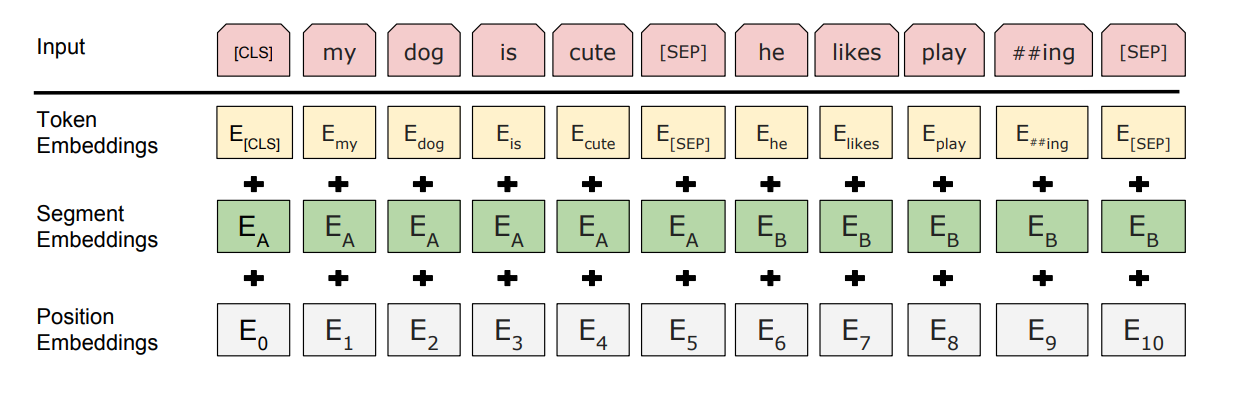
\includegraphics[scale=0.35]{images/bert_embedding_layer.png}
	\caption{BERT Eingabeschicht \cite{BERT:19}}
	\label{embl}
\end{figure}

Aus der Abbildung \ref{embl} kann man nicht nur die Funktion der Schichten lesen, sondern auch ihre Eingaben. In der Token-Embedding-Schicht werden die Tokens der Wörtern gelesen und die Schicht liefert der zugehörige Vektorrepräsentation. Die Segment-Embedding-Schicht erhält den Segmentenvektor, der beim Vorverarbeitung der Eingabepaare erstellt wird. Der Positional-Embedding-Layer codiert die Wortindexen in Vektoren. Die Summe der Ergebnisvektoren aus den einzelnen Schichten liefert den Eingebetteten Vektor, der die Eingabe im Encoder ist. 

\subsubsection{Optimizer und Loss-Funktion}\label{optimizer_and_loss}
Der Nächste Schritt ist die Definition der Optimizer und die Fehlerfunktion. Hier verwende ich den Adaptive-Movement-Optimizer. Laut \cite{CO:19} liefern Adam und RMSProp (\textbf{R}oot \textbf{M}ean \textbf{S}quare \textbf{Prop}agation) bessere Richtigkeit und bessere Fehlerrate als die anderen Optimizers, wie SGD(\textbf{S}tochastic \textbf{G}radient \textbf{D}escent) and AdaGrad(\textbf{Ada}ptiv \textbf{Gra}dients).  
Bei unser ersten Task (Masked Language Processing) wird versucht die maskierten Wörter bestimmt zu werden. Das impliziert, dass jedes maskierte Wort einen aus mehreren Klassen gehören kann, bzw. einen aus vielen Wörtern sein kann. Aus diesem Grund können nur zwei Fehlerfunktionen verwendet werden, die \textit{CategoricalCrossEntropy} und \textit{SparseCategoricalCrossEntropy} sind.

\textit{CategoricalCrossentropy} ist geeignet, wenn die Ausgabe die partielle Zugehörigkeit zu den Klassen ist. \textit{SparseCategoricalCrossentropy} ist besser geeignet, wenn die Ausgabe keinen Vektor aber einen Integerwert ist. Dieser Integer stellt die zugehörige Klasse dar. Welche Fehlerfunktion verwendet wird, hängt nur von der Form der Ausgabe. In unserem Fall habe ich mich für den \textit{CategoricalCrossEntropy} entschieden, da Die Ausgaben einen Softmax-Vektor ist. Später bei der Anpassung \ref{fine_tuning} wird die \textit{SparseCategoricalCrossEntropy} verwendet.

\subsection{Fine-Tuning a BERT-Model}\label{fine_tuning}

Das Model für den Fine-Tuning wurde vom TensorflowHub \cite{tfhub:21} genommen. Es wird ein Model mit den selben Hyperparametern wie das Model aus dem letzten Unterkapitel \ref{bert_class} verwendet. Auf TensorflowHub sind mehrere Modelle zur wiederverwendung, hier unteranderem BERT multilangual Cased Model, BERT English uncased, sowohl das Base-BERT-Model als auch das Large-Model. Dementsprächend kann das geeignete Model für die Task ausgewählt. In meinem Fall will einen Translationmodel aufbauen, für diesen Zweck habe ich das Multilingual BERT-Model \cite{BERTMM:21} genutzt. 

\subsubsection{BERT-Model}

Das gelernte BERT-Model kann wie folgt geladen werden:

\begin{lstlisting}[language=Python, caption={Laden von dem BERT-Model}]
	# directly from the website
	pre_trained_model = 'https://tfhub.dev/tensorflow/bert_multi_cased_L-12_H-768_A-12/4'
	# or from file system
	pre_train_model_path = 'abs/path/to/Model/dir'
	encoder_input = hub.KerasLayer(pre_trained_model, trainable=True, name="BERT_Encoder")
\end{lstlisting}

Das Model kann als eine Schicht geladen und somit in dem Model angefügt werden. Für den Lernprozess braucht das Model eine weitere Schicht, die das Raten darstellen soll. Dafür bietet sich eine einfache Dense-Schicht am Model anzuhängen, die dann die Ausgabe des BERT-Models mit einem Fully Conected Layer verbidet. Die Rolle der Dense-Schicht ist die Ausgabe in der richtige Shape zu verwandeln. Die Ausgabe vom BERT-Model ist einen Vektor mit der Kardinalität \textit{batch\_size} $\times$ \textit{sequence\_length} $\times$ \textit{d\_model}. Die Dense-Schicht verwandelt den Ausgabevektor in der Kardinalität \textit{batch\_size} $\times$ \textit{sequence\_length} $\times$ \textit{vocab\_size}. Die Sequenzgröße entspricht die Länge des Satzes, oder jeder Index beschreibt ein Wort im Satz. Die Variable \textit{d\_model} repräsentiert die Anzahl der Eigenschaften, nach dennen Wörter klassifiziert werden. Die Dense-Schicht verbundet somit die Eingeschaften der einzelnen Worten zu einem Neuron  und die Ausgabe des Neurons ist einen Wert, der für oder gegen einen bestimmten Wort aus dem Wortschatz. Ein weiterer Schritt ist gebraucht, damit diese Werte in Wahrscheinlichkeiten umgewandelt werden und das erfolgt nämlich durch Anwendung der Softmax-Funktion. Das heißt, dass es dem Model gesagt wird, dass es raten soll, wie die Übersetzung des Eingabesatzes lautet. Hier ist das Model gegeben:

\begin{lstlisting}[language=Python, label=BERT_Definition, caption={Definition des BERT-Models zur Anpassung}]
# input Layer with shape=(None, seq_length)
# these are the expected inputs in the BERT model
inputs = dict(
	input_word_ids=tf.keras.layers.Input(shape=(max_sentence_size,), dtype=tf.int32),
	input_mask=tf.keras.layers.Input(shape=(max_sentence_size,), dtype=tf.int32),
	input_type_ids=tf.keras.layers.Input(shape=(max_sentence_size,), dtype=tf.int32)
)
# BERT-Model
encoder_input = hub.KerasLayer(pre_trained_model, trainable=True, name="BERT_Encoder")
outputs = encoder_input(inputs)
net = outputs['sequence_output']
# dropout layer to help prevent overfitting
net = tf.keras.layers.Dropout(0.1)(net)
# dense layer for guessing
output = tf.keras.layers.Dense(vocab_size, activation=None)(net)
# This is our Model
model = tf.keras.Model(inputs, output)
\end{lstlisting}

\subsubsection{Datensatz}
Die Übersetzungstask ähnelt sehr eine Frage-Antwort-Task. Deswegen müssen unsere Datensammlung so vorbereiten, dass wir Satz und Übersetzung gruppieren. Für diese Task habe ich den Datensatz \textit{ted\_hrlr\_translate\_pt\_en\_converter} verwendet. Der Datensatz ist auf dem Google Storage zu finden. In der Datensammlung sind Sätze auf Englisch und Portugiesisch, also wir führen eine Übersetzung vom Englischen ins Portugiesische. Die Datensammlung besteht aus 51785 Sätze jeweils in Englisch und Portugiesisch, insgesamt 103570 Sätze. Die Sätze die über die erlaubte Sequenzlänge sind, werden verworfen. Die Ausgewählte Satzgröße beträgt 128. Da die Höhere Satzlänge eine längeren Lernzeit bedeutet, habe ich in Bezug zu der Hardware, die mir zur Verfügung steht, eine Sequenzlänge von 128 Wörter, inklusive '[CLS]' and '[SEP]' Schlüsselwörter. Das Laden der Datensammlung erfolgt über den folgenden Programmcode:

\begin{lstlisting}[language=Python, caption={Laden der Trainingsdaten}]
	model_name = 'ted_hrlr_translate_pt_en_converter'
	tf.keras.utils.get_file(f"{model_name}.zip", f"https://storage.googleapis.com/download.tensorflow.org/models/{model_name}.zip", cache_dir='.', cache_subdir='', extract=True)
	tokenizer = tf.saved_model.load(model_name)
\end{lstlisting}

Nach der Ausführung des Codes wird die Datensammlung im aktuellen Ordner heruntergeladen und entpackt. Mit Hilfe der dritten Zeile wird der Datensatz zur Nutzung geladen. Der Nächste Schritt ist die Vorbereitung der Sätze für den Lernprozess. Hier Müssen die Eingaben in einem Dictionary gespeichert werden, da das BERT-Model so definiert wird. Wie die Eingabe aussieht, ist in der dritten Zeile aus dem Listing \ref{BERT_Definition} zu erkennen.

\subsubsection{Optimizer und Fehlerfunktion}

Als Nächstes werden die Optimizer und die Fehlerfunktion definiert. Für den Optimizer wird zwar einen Adam-Optimizer, der aber einen Scheduler für die Lernrate besitzt. Das bedeutet, dass die Rate im Laufe des Trainings angepasst wird. Die Konfiguration für den Optimizer ist durch den Programmcode gegeben:

\begin{lstlisting}[language=Python, caption={BERT Optimizer}]
	from official.nlp import optimization
	# learning rate
	init_lr = 5e-5
	# number steps pro epoch
	steps_per_epoch = len(train_input_array)
	# number of warmup stels
	num_warmup_steps = int(0.1 * steps_per_epoch)
	# the optimizer
	optimizer = optimization.create_optimizer(init_lr=init_lr,
	num_train_steps=steps_per_epoch,
	optimizer_type='adamw')
\end{lstlisting}

Die genutzte Fehlerfunktion ist SparceCategoricalCrossEntropy. Der Grund dafür ist die Struktur des Labels und die Ausgabe des Models (siehe Erklärung im Unterkapitel \ref{optimizer_and_loss}). Die Fehlerfunktion hat keine besonderen Konfiguration, außer einen Parameter $\textit{from\_logits}$ der auf True gesetzt wird. Dadurch wird der Fehlerfunktion gesagt, dass keine Softmax im Voraus angewendet wird. Dementsprechend wird eine Sotfmax-Funktion zuerst ausgeführt, bevor die Fehlerrate errechnet wird.
